\twocolumn[{%
	\renewcommand\twocolumn[1][]{#1}%
	\maketitle
	\begin{center}
		\newcommand{\teaserwidth}{\textwidth}
		% \vspace{-0.15in}
		\centerline{
			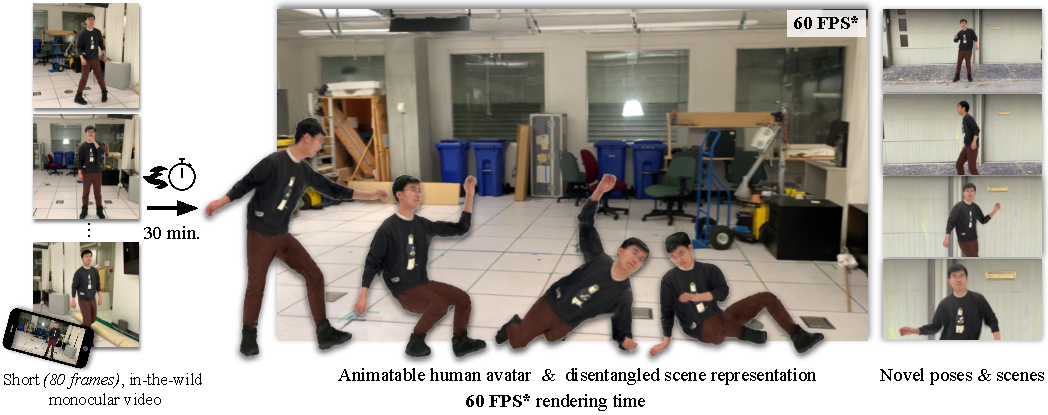
\includegraphics[width=\teaserwidth,clip]{figures/pdf_files/teaser_v2.pdf}
		}
		\vspace{-1ex}
		\captionof{figure}{\textbf{Human Gaussian Splats (\acronym)} is a neural rendering framework that trains on 50-100 frames of a monocular video containing a human in a scene. HUGS enables novel view rendering with novel human poses at \textbf{60 FPS} by learning a disentangled representation that can also render the human in other scenes.  \textcolor{magenta}{\textbf{*}Main submission indicates runtime speed as 32 FPS. During SupMat submission we have found out a bug causing slow performance. After resolving the issue, actual speed becomes 60 FPS.} }
		% \vspace{-0.08in}
		\label{fig:teaser}
	\end{center}%
}]